\section{simulation}
\label{sec:simulation}

\subsection{simulator}
We developed a simulator that models the behaviour of guests flows in a crowd-shared network connected through a wireless mesh network. The simulator uses TFA wireless mesh topology which consists of 21 nodes. In our simulator, each TFA node represents an access home router with 16 Mbps internet access capacity, whereas each mesh link has the capacity a IEEE 802.11ac wireless link with 40 Mhz bandwidth and 200 Mbps data rate. 

To model sharing policy of of access routers owners, the simulator switches the routers ON and OFF for certain time period during the simulation lifetime. The length of the ON and OFF period are randomly generated out of two exponential distribution with different means (555 mintues for OFF period and 106 minutes for the ON period ). The means are driven out of real world data of home routers owners behaviour. To account for the ON or OFF period, the simulator equip each router with a timer to record how long a router has been ON of OFF. The simulator distinguish between ON and OFF through a boolean flag which is true when the router is ON and False when the router is OFF. 

To reflect real world traffic, we consider dynamic communication pattern where guests flows arrive to and departure from the network at certain time points. Flow arrival rates and flows durations are generated based on Poisson and exponential distribution, respectively. Each flow has constant bit rate which is sampled out of a uniform distribution. Since in reality the flows load across the home routers may differ due to the number of guests connected to each router, we use geometric distribution to randomly choose at which router the next flow will arrive. 

To grant internet access to the flows, we simulate two methods. In the first case, we only give access to flows through the router at which they arrived given that there is enough internet access capacity, this method ignores the mesh network. In the second method, we take into account the mesh network. In other words, if there is no enough capacity in the local access router, the flow is redirected to another router in the network. We choose the router to which the flow is redirected based on worst-fit decreasing algorithm. The algorithm starts by sorting the flows to be redirected in non-decreasing order of their rate. Then, starting from the flow with the highest rate, for each flow the algorithm tries to find the router with with the highest available internet access capacity. The worst-fit decreasing algorithm is also used to redirect flows when a router goes OFF to sustain as much as possible flows in the network and reduce disruption by the routers owners sharing policy.
%Furthermore, to show performance of the system under dynamic communication pattern, we consider flows with limited life time which arrive and leave the system at certain time point.   

The simulation proceeds in discrete time ticks. At each time tick, the simulator updates the ON/OFF timer of the access routers and subsequently switches the routers with expired timer ON or OFF depending on their current status. It also removes flows which expired and generates new flows if required. Furthermore, it assigns flows to home access routers or redirect flows between different access points in case they can not be accommodated locally using the decreasing worst-fit algorithm. 

Due to the larger mean of the ON and OFF period (8 hours OFF and 1.5 hours ON), we run each simulation for 60 Hours with the time scale of 20 minutes. 

To evaluate the benefits of mesh network, we measure the average link utilization and of the access router as well as the accumulated acceptance rate of the network at each time tick.  For link utilization, only routers which are ON are taken into account. The acceptance rate represents the number of finished flows/divided by the number of flows served by the network. 

 
\subsection{Simulation Results}
 
%\begin{figure}[t]
%\begin{center}
%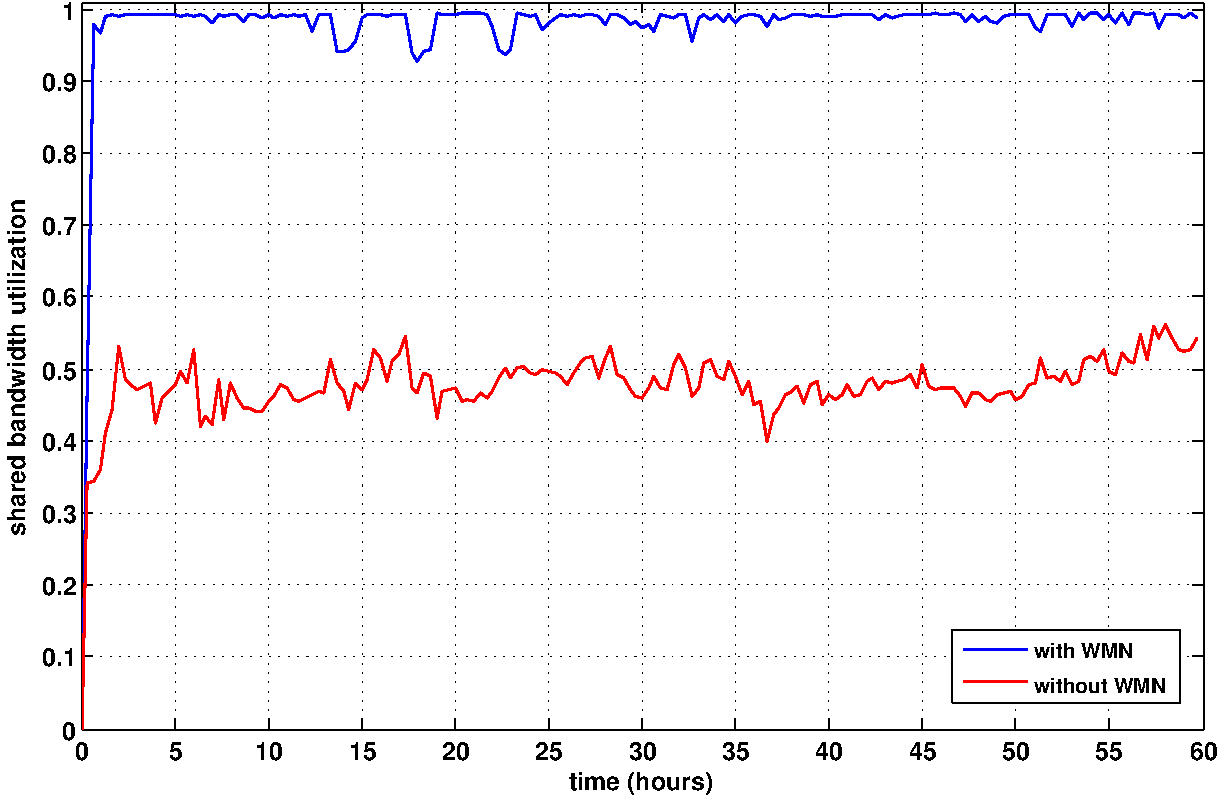
\includegraphics[width=0.6\linewidth]{results/utilization.pdf}  
%\caption{Network processing architecture components.}
%\label{fig:architecture}
%\end{center}
%\vspace{-7mm}
%\end{figure}
%
%Evaluation results shows that 
%\vspace{3mm}
%
%\begin{figure}[t]
%\begin{center}
%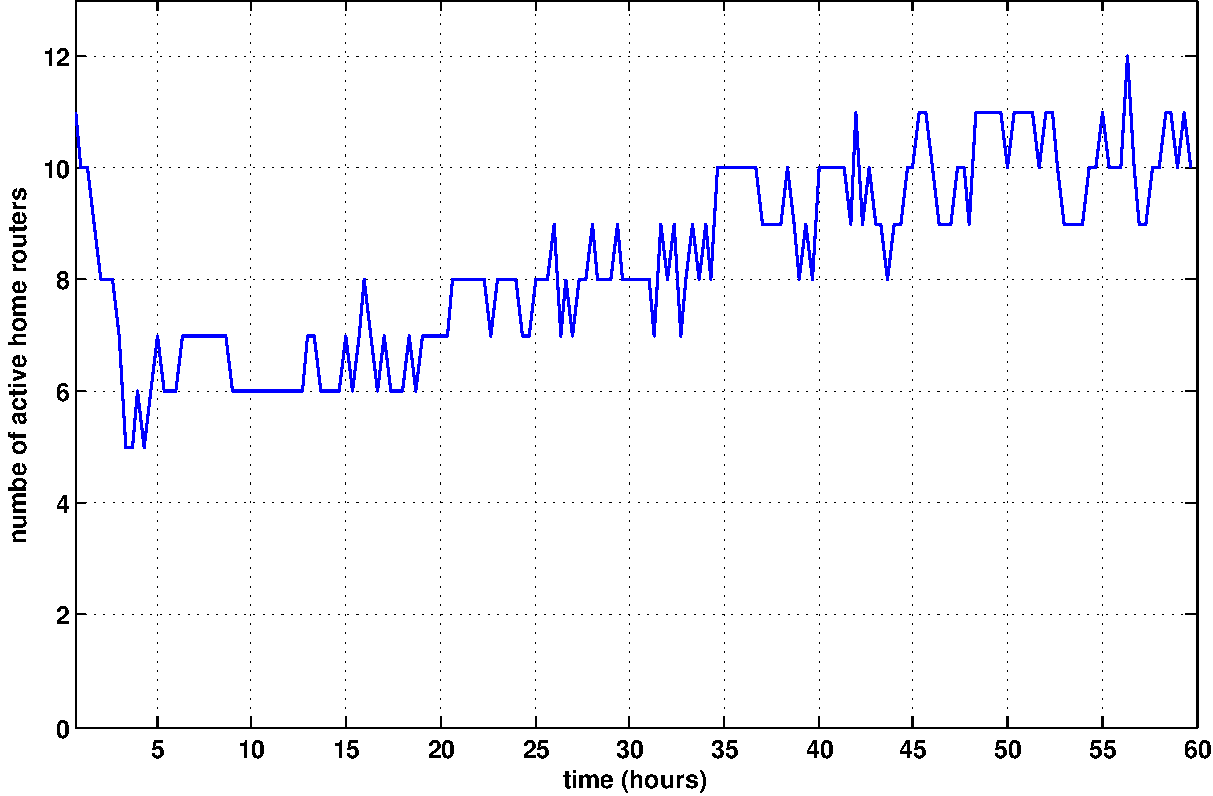
\includegraphics[width=0.6\linewidth]{results/on_routers.pdf}  
%\caption{Network processing architecture components.}
%\label{fig:architecture}
%\end{center}
%\vspace{-7mm}
%\end{figure}
%
%
%\begin{figure}[t]
%\begin{center}
%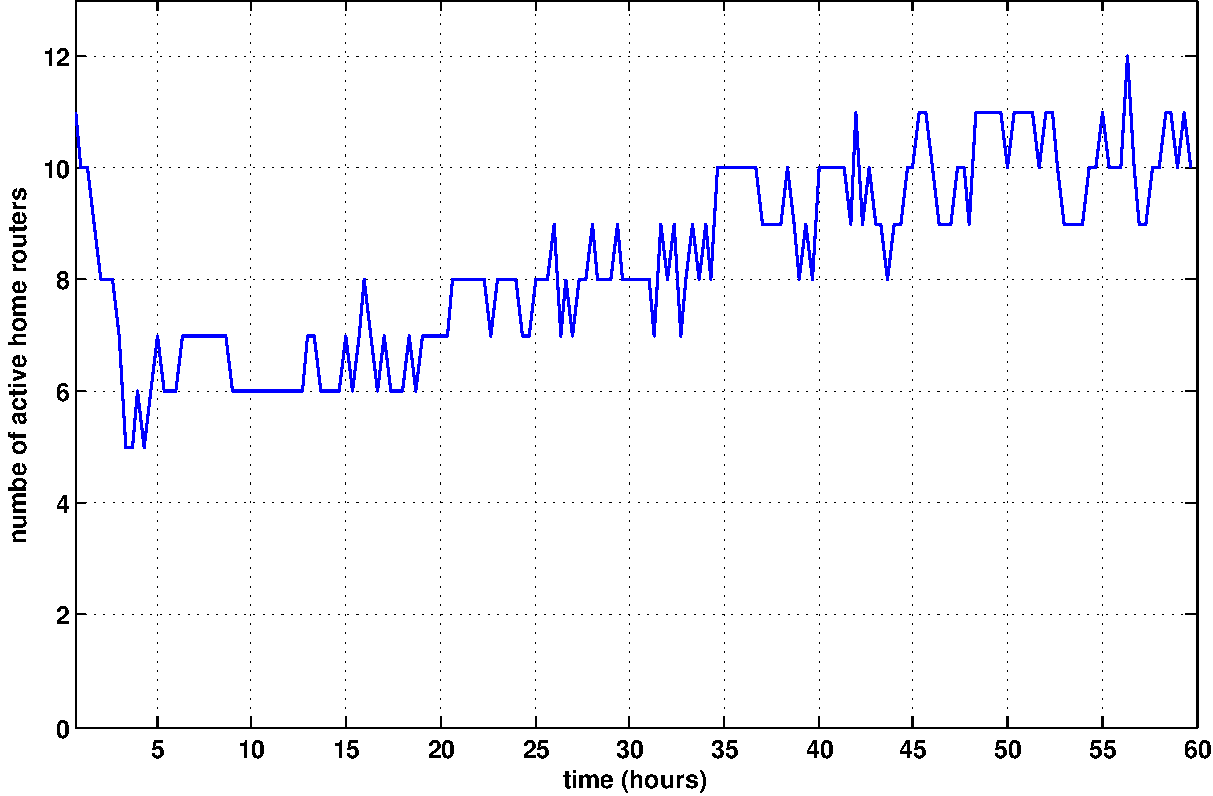
\includegraphics[width=0.6\linewidth]{results/on_routers.pdf}  
%\caption{Network processing architecture components.}
%\label{fig:architecture}
%\end{center}
%\vspace{-7mm}
%\end{figure}

\subsection{Simulation Results}

